\capitulo{3}{Conceptos teóricos}

La parte del proyecto con mayor complejidad teórica radica en el
algoritmo de visión artificial, el cual se puede dividir en cuatro
fases. En primer lugar, se realiza un preprocesado de la señal de
entrada para optimizarla. En segundo lugar, se substrae el fondo para
segmentar los objetos en movimiento. Posteriormente, se realiza un
posprocesado de la señal para mejorar los resultados obtenidos de la
substracción del fondo. Y por último, se clasifican y cuentan los
contornos que pueden pertenecer a una abeja.

A continuación se exponen los conceptos teóricos que conlleva cada fase.

\section{Preprocesado}\label{preprocesado}

Antes de aplicar el algoritmo de substracción del fondo, es recomendable
realizar un preprocesado de los fotogramas para facilitar el procesado
posterior, minimizar el ruido y optimizar los resultados. A continuación
se explican las técnicas utilizadas.

\subsection{Conversión de RGB a escala de grises}\label{conversion-de-rgb-a-escala-de-grises}

Los fotogramas captados por la cámara se devuelven en formato RGB. En
este formato se poseen tres matrices, una por cada canal
(\emph{Red-Green-Blue}). La suma aditiva de los tres canales resulta en
una imagen a color.

Sin embargo, el color no proporciona ninguna información relevante en
nuestra tarea de identificación de abejas. Es por esto que se pueden
convertir los fotogramas de RGB a escala de grises. De esta manera, se
trabajará solamente con una matriz de píxeles en lugar de tres.
Simplificando, en gran medida, el número de operaciones a realizar y por
tanto, aumentado el rendimiento de nuestro algoritmo final.

OpenCV utiliza la conversión colométrica a escala de grises
\citep{opencv:color_cvt}. Esta técnica se basa en principios
colométricos para ajustar la luminancia de la imagen a color y la imagen
resultante. Devolviendo una imagen con la misma luminancia absoluta y la
misma percepción de luminosidad \citep{wiki:grayscale}.

Utiliza la siguiente fórmula para calcular la luminancia resultante:

\begin{equation*}
    \text{RGB[A] to Gray:} \quad Y \leftarrow 0.299 \cdot R + 0.587 \cdot G + 0.114 \cdot B
\end{equation*}

La fórmula calcula la luminancia de una forma no lineal, sin necesidad
de realizar una expansión \emph{gamma}. Los coeficientes intentan imitar la
percepción de intensidad medida por un humano tricromático, siendo más
sensible al color verde y menos al color azul \citep{wiki:grayscale}.

\subsection{Desenfoque Gaussiano}\label{desenfoque-gaussiano}

Las imágenes captadas pueden contener ruido que puede dificultar su
procesamiento. El ruido son variaciones aleatorias del brillo o del
color de una imagen. Una técnica que permite reducirlo es el desenfoque.

En nuestro caso hemos utilizado desenfoque Gaussiano, un filtro de paso
bajo que reduce las componentes de alta frecuencia de la imagen
utilizando para ello una convolución con una función Gaussiana
\citep{wiki:gaussian}. Se diferencia del desenfoque promedio en que da
más peso a los vecinos cercanos, siendo estos más influyentes en el
resultado.

El \emph{kernel} utilizado en la convolución es una muestra discreta de una
función Gaussiana. En nuestro caso utilizamos un \emph{kernel} $3 \times 3$ que se
corresponde con: \citep{book:mastering_opencv}

\begin{equation*}
    M = 
    \begin{bmatrix}
    1 & 2 & 1 \\[0.3em] 
    2 & 4 & 2 \\[0.3em] 
    1 & 2 & 1
    \end{bmatrix}
\end{equation*}

En la imagen \ref{fig:s1} se puede ver el resultado de aplicar esta fase a
la imagen de entrada:

\imagen{s1}{Resultado de la fase de preprocesado.}

\section{Substracción del fondo}\label{substraccion-del-fondo}

En un sistema de monitorización por vídeo resulta de gran interés el
poder extraer los objetos en movimiento del resto de la imagen. Esto se
conoce como extracción del fondo, en inglés \emph{background
subtraction} o \emph{foreground detection}, y consiste en clasificar
todos los píxeles de un determinado fotograma bien como fondo, o como
primer plano \citep{wiki:bs}. En primer plano se engloban todos los
objetos en movimiento, mientras que en el fondo se encuentran todos los
objetos estáticos junto con posibles sombras, cambios de iluminación u
otros objetos en movimiento que no son de interés, como puede ser la
rama de un árbol balanceándose por el viento. Se trata de un paso
crítico, ya que algoritmos posteriores dependen en gran medida de los
resultados de este.

En nuestro proyecto, la toma de imágenes se realiza mediante una cámara
estática. Esto facilita en parte la detección del fondo, ya que este se
corresponderá con todos los píxeles estáticos. Sin embargo, como
trabajamos en un entorno al aire libre, tenemos que lidiar también con
cambios de iluminación, sombras, u otros objetos móviles que no son de
nuestro interés (falsos positivos).

Con OpenCV para Android podemos implementar varios algoritmos básicos de
extracción del fondo y además, nos proporciona la implementación de dos
algoritmos más sofisticados: \texttt{BackgroundSubtractorMOG2} y \\
\texttt{BackgroundSubtractorKNN}. 

Tras realizar un estudio de todos
ellos, nos decantamos finalmente por \texttt{BackgroundSubtractorMOG2}.
A continuación, explicamos el funcionamiento de todos los algoritmos que
se probaron, así como los resultados que proporcionaron.

\subsection{Substracción con imagen de referencia}\label{substraccion-con-imagen-de-referencia}

Se parte de una imagen de referencia del fondo, en la que no haya ningún
objeto en movimiento. A partir de esta, se obtienen los elementos en
movimiento substrayendo a cada fotograma la imagen tomada como
referencia.

Este método, al tomar un modelo del fondo tan sencillo y estático, es
muy vulnerable a cambios en la escena (iluminación, sombras, objetos del
fondo con ligeros movimientos, pequeñas oscilaciones de la cámara,
etc.). Sin embargo, ofrece muy buenos resultados cuando se trabaja en
una escena con la iluminación y los elementos controlados, ya que al ser
tan simple, es muy eficiente \citep{programarfacil:detmov}.

Para implementar este algoritmo con OpenCV, se hace uso de la función
\texttt{Core.absdiff()}.

En nuestro problema, al trabajar al aire libre nos es imposible utilizar
este algoritmo. Ya que el modelo del fondo cambia constantemente.

\subsection{Substracción del fotograma anterior}\label{substraccion-del-fotograma-anterior}

En este método, el modelo del fondo se extrae del fotograma anterior. De
tal manera, que a cada nuevo fotograma se le substrae el anterior.

De esta manera se mejora la respuesta a cambios en la escena, como los
cambios de iluminación. Sin embargo, si un objeto en movimiento se queda
estático en la imagen, este deja de ser detectado
\citep{book:opencv_java}.

La implementación se realiza como en la técnica anterior, variando el
modelo del fondo.

Tras probarlo en nuestro problema específico, vimos que no nos era de
utilidad. Ya que el fotograma resultante de la diferencia contenía las
abejas por duplicado (la abeja en el fotograma actual y misma abeja en
el fotograma anterior en otra posición).

\subsection{Substracción del acumulado de los fotogramas anteriores}\label{substraccion-del-acumulado-de-los-fotogramas-anteriores}

Una mejora interesante del algoritmo anterior supone tomar como modelo
del fondo un acumulado de los fotogramas anteriores de acuerdo a un
ratio de aprendizaje. De esta forma, se puede lidiar con cambios en el
fondo de la imagen dinámicamente. El modelo se calcula de acuerdo a la
siguiente fórmula:

\begin{equation*}
    u_t = (1-\alpha )u_{t-1}+\alpha\ p_t
\end{equation*}

Donde $p_t$ es el nuevo valor del píxel, $u_{t-1}$ es la media del
fondo en el instante $t-1$, $u_t$ es la nueva media del fondo y
$\alpha$ es el ratio de aprendizaje (cómo de rápido olvida los \emph{frames}
anteriores) \citep{book:opencv_java}.

OpenCV provee la función \texttt{Imgproc.accumulateWeighted()} que
implementa la fórmula anterior por nosotros. Haciendo uso de esta
función y de la utilizada en la sección anterior podemos implementar
este algoritmo.

Tras probarlo, vimos que tenía una eficiencia muy buena y se adaptaba a
los cambios correctamente. Sin embargo, no era capaz de diferenciar las
sombras de las abejas, por lo que se obtenían falsos positivos.

\subsection{BackgroundSubtractorKNN}\label{backgroundsubtractorknn}

Se trata de un método que se basa en el algoritmo de clasificación
supervisada \emph{K Nearest Neighbors} (k-nn). El algoritmo fue
propuesto en el artículo \citep{art:zivkovic_efficient_2006}. Y de
acuerdo con sus conclusiones, es muy eficiente cuando el número de
píxeles que se corresponden con el primer plano es bajo.

La clase de OpenCV que lo implementa es
\texttt{BackgroundSubtractorKNN}. Los parámetros más importantes son:

\begin{itemize}
\tightlist
\item
  \texttt{history}: número de fotogramas recientes que afectan al modelo
  del fondo.
\item
  \texttt{dist2Threshold}: umbral de la distancia al cuadrado entre el
  píxel y la muestra para decidir si un píxel está cerca de esa muestra.
\item
  \texttt{detectShadows}: con un valor verdadero detecta las sombras
  (aumenta considerablemente el tiempo de procesado).
\end{itemize}

En nuestras pruebas, el algoritmo proporcionaba unos resultados buenos
pero su tiempo de ejecución era muy elevado (entorno a 25ms/frame). Como
el tiempo de ejecución es un factor clave en nuestro proyecto, se
descartó el uso de este algoritmo.

\subsection{BackgroundSubtractorMOG2}\label{backgroundsubtractormog2}

\texttt{BackgroundSubtractorMOG2} es una mejora del algoritmo
\\ \texttt{BackgroundSubtractorMOG}. En la versión original de OpenCV se
encuentran implementados ambos, sin embargo, en los \emph{wrappers} para
Android solo disponemos de la revisión.

\texttt{BackgroundSubtractorMOG} está basado en el modelo \emph{Gaussian
Mixture} (GMM). Se trata de un modelo compuesto por la suma de varias
distribuciones Gaussianas que, correctamente elegidas, permiten modelar
cualquier distribución \citep{coursera:gmm}.

El algoritmo de substracción del fondo fue propuesto en el artículo
\citep{art:yao_improved_2001} y modela cada píxel del fondo como la
mezcla de \emph{K} distribuciones Gaussianas. Los pesos de la mezcla
representan las proporciones de tiempo que el color de ese píxel se ha
mantenido en la escena. Siendo los colores de fondo más probables los
que más permanezcan y sean más estáticos \citep{opencv:bs_tutorial}.

\texttt{BackgroundSubtractorMOG2} se basa en los mismos principios que
su antecesor pero implementa una mejora sustancial. Es el propio
algoritmo el que selecciona el número adecuado de distribuciones
Gaussianas necesarias para modelar cada píxel. De esta manera, se mejora
notablemente la adaptabilidad del algoritmo a variaciones en la escena.
Fue propuesto en los artículos \citep{art:zivkovic_improved_2004} y
\citep{art:zivkovic_efficient_2006}.

El código fuente de este algoritmo está disponible en 
\citep{github:background_segm} (interfaz) y
\citep{github:bgfg_gaussmix2} (implementación).

La clase de OpenCV que lo implementa es
\texttt{BackgroundSubtractorMOG2}. Posee los siguientes parámetros
configurables: \citep{opencv:mog2}

\begin{itemize}
\tightlist
\item
  \texttt{history}: número de fotogramas recientes que afectan al modelo
  del fondo. Se representa en la literatura como \texttt{T}. Por
  defecto, 500 fotogramas. Nosotros hemos obtenido buenos resultados con
  valores de entorno a 50.
\item
  \texttt{learningRate}: valor entre 0 y 1 que indica como de rápido
  aprende el modelo. Si se establece un valor de -1 el algoritmo elige
  automáticamente el ratio. 0 significa que el modelo del fondo no se
  actualiza para nada, mientras que 1 supone que el modelo del fondo se
  reinicializa completamente cada nuevo fotograma. En la literatura
  podemos encontrar este parámetro como \texttt{alfa}. Si el intervalo
  que se quiere considerar es \texttt{history}, se debe establecer
  \texttt{alfa=1/history} (valor por defecto). También se pueden mejorar
  los resultados iniciales estableciendo \texttt{alfa=1} en el instante
  0 e ir decrementándolo hasta \texttt{alfa=1/history}. De esta manera,
  en el inicio aprende rápidamente, pero una vez estabilizada la
  situación las variaciones afectan menos al modelo. En nuestro caso, el
  valor por defecto ha funcionado correctamente.
\item
  \texttt{backgroundRatio}: si un pixel del primer plano permanece con
  un valor semi-constante durante \texttt{backgroundRatio*history}
  fotogramas, es considerado fondo y se añade al modelo del fondo como
  centro de una nueva componente Gaussiana. En los artículos se hace
  referencia a este parámetro como \texttt{TB}. \texttt{TB=0.9} es el
  valor por defecto. Este parámetro nos permite decidir cuando dejar de
  contar una abeja que se ha quedado inmóvil o un objeto nuevo en la
  escena como podría ser una hoja que se acaba de caer de un árbol.
\item
  \texttt{detectShadows}: con un valor verdadero (valor por defecto)
  detecta las sombras (aumenta ligeramente el tiempo de procesado). Nos
  permite despreciar las sombras de las abejas con muy buenos
  resultados.
\item
  \texttt{shadowThreshold}: el algoritmo detecta las sombras comprobando
  si un píxel es una versión oscurecida del fondo. Este parámetro define
  cómo de oscura puede ser la sombra como máximo. Por ejemplo, un valor
  de 0.5 (valor por defecto) significa que si un píxel es más del doble
  de oscuro, entonces no se considerará sombra. En los artículos se
  representa como \texttt{Tau}.
\item
  \texttt{shadowValue}: es el valor utilizado para marcar los píxeles de
  sombras en la máscara resultante. El valor por defecto es 127. En la
  máscara devuelta, un valor de 0 siempre se corresponde con un pixel
  del fondo, mientras que un valor de 255 con un píxel del primer plano.
\item
  \texttt{nMixtures}: número máximo de componentes Gaussianas para
  modelar el modelo del fondo. El número actual se determina
  dinámicamente para cada píxel. Hemos utilizado el valor por defecto,
  5.
\item
  \texttt{varThreshold}: umbral utilizado en el cálculo de la distancia
  cuadrada de Mahalanobis entre el píxel y el modelo del fondo para
  decidir si una muestra está bien descrita por el modelo o no. Este
  parámetro no afecta a la actualización del modelo del fondo. Se
  representa como \texttt{Cthr}. Por defecto, 16. Se han obtenido
  mejores resultados con valores de entorno a 40.
\item
  \texttt{varThresholdGen}: umbral sobre la distancia cuadrada de
  Mahalanobis entre el píxel y el modelo para ayudar a decidir si un
  píxel está cercano a alguna de las componentes del modelo. Si no es
  así, es considerado como primer plano o añadido como centro de una
  nueva componente (dependiendo del \texttt{backgroundRatio}). Se
  representa como \texttt{Tg} y su valor por defecto es 9. Un valor
  menor genera más componentes Gaussianas, mientras que un valor mayor
  genera menos.
\item
  \texttt{complexityReductionThreshold}: este parámetro define el número
  de muestras necesarias para probar que una componente existe. Se
  representa como \texttt{CT}. Su valor por defecto es \texttt{CT=0.05}.
  Si se establece su valor a 0 se obtiene un algoritmo similar al de
  Stauffer \& Grimson (no se reduce el número de componentes).
\item
  \texttt{varInit}: varianza inicial de cada componente Gaussiana.
  Afecta a la velocidad de adaptación. Se debe ajustar teniendo en
  cuenta la desviación estandar de las imágenes. Por defecto es 15.
\item
  \texttt{varMin}: varianza mínima. Por defecto, 4.
\item
  \texttt{varMax}: varianza máxima. Por defecto, \texttt{5*varInit}.
\end{itemize}

De todos ellos, los parámetros más importantes a ajustar son
\texttt{history} o \texttt{learningRate}, \texttt{varThreshold} y
\texttt{detectShadows}.

La parametrización correcta de este algoritmo es clave para su buen
funcionamiento. Por ello, durante las pruebas se desarrolló una
aplicación Java que permitía variar todos estos parámetros en 
tiempo real, ver la salida de cada fase y 
calcular los tiempos de ejecución. De esta manera, se pudo elegir 
la mejor configuración para nuestro problema concreto.

Una vez parametrizado correctamente, vimos como este algoritmo era el
que mejores resultados nos proporcionaba. Con un tiempo de ejecución en
nuestro equipo de pruebas de entorno a 4 ms/frame, mucho menor que el
proporcionado por \texttt{BackgroundSubtractorKNN}, de entorno a
25 ms/frame. El algoritmo detectaba correctamente las abejas, era
resistente al ruido, y además, era capaz de diferenciar una abeja de su
sombra. Por todos estos motivos, se seleccionó para la fase de
substracción del fondo.

En la imagen \ref{fig:s2} se puede ver el resultado de aplicar
\\ \texttt{BackgroundSubtractorMOG2} a la salida de la fase anterior:

\imagen{s2}{Resultado de la fase de substracción del fondo.}

Se puede apreciar como ha descartado correctamente las sombras en
movimiento de los árboles y se ha quedado únicamente con los objetos en
movimiento.

\section{Posprocesado}\label{posprocesado}

Para mejorar los resultados de la extracción de fondo y preparar la
imagen para la búsqueda de contornos, se han aplicado las siguientes
técnicas:

\subsection{Dilatación}\label{dilatacion}

Se trata de una operación morfológica por la cual se expanden las
regiones luminosas de una imagen. Esto se consigue mediante la
sustitución de cada píxel por el más brillante de los vecinos
considerados por el \emph{kernel} (matriz utilizada para la
convolución) \citep{book:mastering_opencv}. De esta manera se 
consiguen unir las regiones de abejas que podían haberse roto.

\subsection{Erosión}\label{erosion}

Se trata de la operación contraria a la anterior, expande las regiones
oscuras de la imagen. Para ello se coge el valor mínimo de los valores
considerados por el \emph{kernel} \citep{book:mastering_opencv}.

La dilatación nos permite reconstruir las abejas, pero también aumenta
su tamaño, aumentando el riesgo de solapamientos. Para evitar esto, se
vuelve a reducir el tamaño de estas mediante una erosión.

En nuestro algoritmo aplicamos tres operaciones morfológicas seguidas:

\begin{enumerate}
\def\labelenumi{\arabic{enumi}.}
\tightlist
\item
  \textbf{Erosión (3x3)}: elimina las patas de las abejas.
\item
  \textbf{Dilatación (2x2)}: junta la cabeza de las abejas con su cuerpo
  que en numerosas ocasiones es separado durante la substracción de
  fondo.
\item
  \textbf{Erosión (3x3)}: recupera el tamaño inicial.
\end{enumerate}

En la imagen \ref{fig:s3} podemos ver el resultado de esta fase:

\begin{figure}[H]
	\centering
	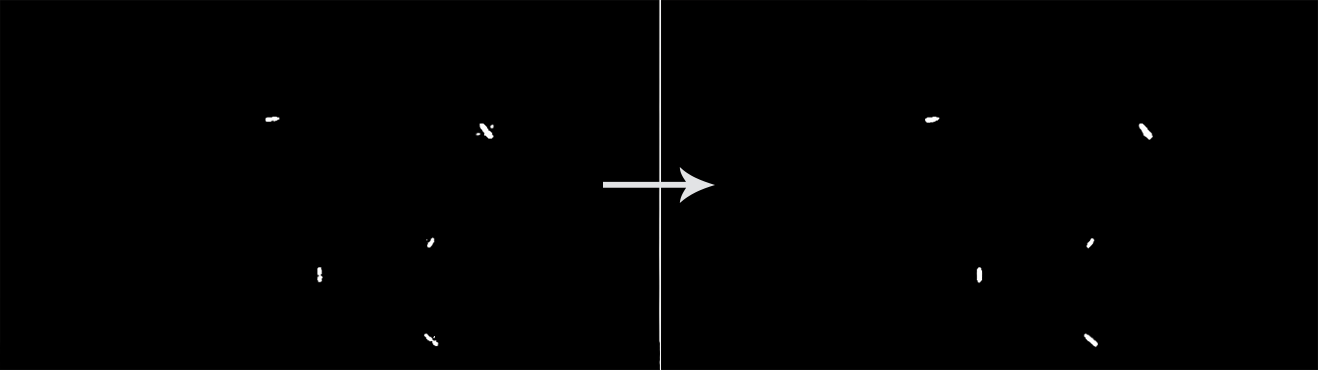
\includegraphics[width=0.9\textwidth]{s3}
	\caption{Resultado de la fase de posprocesado.}
	\label{fig:s3}
\end{figure}

\section{Detección y conteo de abejas}\label{deteccion-y-conteo-de-abejas}

El último paso que realiza nuestro algoritmo de visión artificial es
detectar cuáles de las regiones obtenidas en la fase anterior se
correponden con abejas. Para ello, se realiza una búsqueda de contornos
y se filtran por área.

Entendemos por contorno una línea curva que une todos los puntos
continuos del borde de una región de un mismo color o intensidad.

La salida de la fase anterior es una imagen binaria con los objetos en
movimiento en blanco y el fondo en negro. Por lo tanto, el objetivo de
esta fase es detectar todas las regiones blancas que puedan
corresponderse con una abeja.

OpenCV provee la función \texttt{Imgproc.findContours()} para realizar
la búsqueda de contornos. Esta toma una imagen binaria y devuelve una
lista con todos los contornos encontrados. Para entender la función se
necesita comprender una serie de conceptos: \citep{opencv:contours}

\begin{itemize}
\tightlist
\item
  \textbf{Jerarquía}: los contornos pueden ser independientes unos de
  otros, o poseer una relación padre-hijo cuando un contorno está dentro
  de otro. En la jerarquía se especifican las relaciones entre
  contornos.
\item
  \textbf{Modo de obtención del contorno}: define cómo se van a obtener
  los contornos en cuestión de jerarquía \citep{opencv:find_contours}.

  \begin{itemize}
  \tightlist
  \item
    \texttt{RETR\_LIST}: devuelve todos los contornos en una lista, sin
    ninguna información de jerarquía entre ellos.
  \item
    \texttt{RETR\_EXTERNAL}: devuelve todos los contornos externos. Si
    algún contorno tiene contornos hijo, estos son ignorados.
  \item
    \texttt{RETR\_CCOMP}: devuelve los contornos agrupados en dos
    niveles de jerarquía. Un primer nivel en el que se encuentran todos
    los contornos exteriores. Y un segundo nivel con los contornos
    correspondientes a agujeros en los primeros.
  \item
    \texttt{RETR\_TREE}: devuelve todos los contornos creando un árbol
    completo con la jerarquía.
  \end{itemize}
\item
  \textbf{Método de aproximación de los contornos}: define el método que
  utiliza la función para almacenar los contornos
  \citep{opencv:find_contours}.

  \begin{itemize}
  \tightlist
  \item
    \texttt{CHAIN\_APPROX\_NONE}: almacena todos los puntos del borde
    del contorno.
  \item
    \texttt{CHAIN\_APPROX\_SIMPLE}: almacena sólo los puntos relevantes
    del contorno. Por ejemplo, si el contorno es una línea no se
    necesita almacenar todos los puntos de esta, con el punto inicial y
    el final basta. Esto es lo que realiza este método, eliminar todos
    los puntos redundantes y comprimirlos para que ocupe menos espacio.
  \item
    \texttt{CV\_CHAIN\_APPROX\_TC89\_L1} y
    \texttt{CV\_CHAIN\_APPROX\_TC89\_KCOS}: aplican el algoritmo de
    aproximación de cadena de Teh-Chin, simplificando los polígonos que
    forman los contornos.
  \item
    \texttt{CV\_CHAIN\_CODE}: almacena los contornos utilizando el
    código de cadenas de Freeman.
  \end{itemize}
\end{itemize}

En nuestro caso, la configuración más adecuada es utilizar
\texttt{RETR\_EXTERNAL} y \texttt{CHAIN\_APPROX\_SIMPLE}. Ya que no nos
interesa ningún contorno interno que pueda tener la abeja (y que en
principio no debería tener) y tampoco nos es relevante el cómo se
almacenan estos, sólo nos interesa el número.

Para evitar posibles falsos positivos, establecemos un umbral mínimo y
máximo en el área del contorno. De esta manera, evitamos que contornos
diminutos o grandes generados por ruidos o por objetos del entorno
(moscas, pájaros, roedores\ldots{}) sean contados como abejas.

En la imagen \ref{fig:s4} podemos ver la salida del algoritmo:

\imagen{s4}{Resultado de la fase de detección y conteo de abejas.}

En \ref{fig:flies} se puede apreciar cómo se descartan las tres moscas que hay
en la imagen ya que su área es inferior al área mínima:

\imagen{flies}{Resultado del algoritmo en una imágen con moscas.}
